\documentclass[12pt,a4paper]{article}

%------------------------------------------------
% Packages
%------------------------------------------------
\usepackage[T1]{fontenc}
\usepackage{lmodern}
\usepackage{graphicx}
\usepackage{amsmath,amssymb}
\usepackage{siunitx}
\usepackage{geometry}
\usepackage{fancyhdr}
\usepackage{booktabs}
\usepackage{caption}
\usepackage{float}
\usepackage{subcaption}
\usepackage[dvipsnames]{xcolor}
\usepackage{array}
\usepackage{setspace}
\usepackage[hidelinks]{hyperref}
\usepackage[backend=biber,style=numeric]{biblatex}

\addbibresource{references.bib}

%------------------------------------------------
% Page layout
%------------------------------------------------
\geometry{
    top=1in,
    bottom=1.2in,
    left=1in,
    right=1in
}

\setlength{\headheight}{15pt}
\setlength{\parskip}{0.4em}
\setlength{\parindent}{0pt}

\pagestyle{fancy}
\fancyhf{}
\fancyhead[L]{Ian Cullinane}
\fancyhead[R]{Balmer Series}
\fancyfoot[C]{\thepage}

\sisetup{
    inter-unit-product = \cdot,
    uncertainty-mode = separate,
    per-mode = symbol
}

%------------------------------------------------
% Title
%------------------------------------------------
\title{
    \Large\textbf{Investigation of the Balmer Series}\\[0.5em]
    \large PY2107 -- Experiment 7
}

\author{
    Ian Cullinane -- \textit{125413342}\\[0.5em]
    Lab Partner: Fionn Lichtsinn Doyle\\[0.5em]
    Demonstrators: Jonathan and Olivia
}

\date{14th October 2026}

\begin{document}

\maketitle
\thispagestyle{empty}

\newpage
\tableofcontents
\newpage

%================================================
\section{Abstract}
%================================================

The visible Balmer spectrum of hydrogen was measured with a
diffraction grating. Wavelengths for three spectral lines were
calculated from diffraction-angle readings in orders one to three
and fitted to the Rydberg relation. An unweighted linear fit gave
$R_H=(1.03\pm0.06)\times10^7\ \si{\per\metre}$, 6.21\% below
the infinite-nuclear-mass reference value. The fitted series-limit
wavelength and energy were $389\pm22\ \si{\nano\metre}$ and
$3.2\pm0.2\ \si{\electronvolt}$, respectively. Although the
fit intercept is consistent with zero, the weighted fit has a
reduced chi-squared of 13.46 ($12$ degrees of freedom), indicating
that the adopted measurement uncertainties do not explain all the
observed scatter. The data are broadly consistent with the
Balmer-series model, but the precision is limited by scatter and
systematic uncertainty.

\newpage

%================================================
\section{Theory}
%================================================


The Balmer series of hydrogen arises when electrons transition
from higher energy levels to the final level $n_f=2$, emitting
photons in the visible region of the electromagnetic spectrum.
The wavelengths are described by the Rydberg equation
\cite{py2107,nistRydberg}:

\[
\frac{1}{\lambda}
= R_H \left(\frac{1}{n_f^2}-\frac{1}{n_i^2}\right),
\]

where $\lambda$ is the wavelength of the emitted photon,
$n_i$ and $n_f$ are the initial and final principal quantum
numbers, respectively, and $R_H$ is the Rydberg constant
for hydrogen.

The theoretical hydrogen Rydberg constant accounts for the
finite mass of the nucleus through the reduced mass:

\[
R_H = \frac{m_r}{m_e}R_\infty,
\qquad
m_r = \frac{m_e m_p}{m_e+m_p},
\]

where $m_e$ and $m_p$ are the electron and proton masses,
and $R_\infty$ is the Rydberg constant for an infinitely
heavy nucleus. The CODATA value used here is
$R_\infty=1.0973731568\times10^7\ \si{\per\metre}$
\cite{nistRydberg}.
Applying the reduced-mass correction gives
$R_H=1.096776\times10^7\ \si{\per\metre}$ for hydrogen.

A diffraction grating is used to determine the wavelength
of each spectral line. The grating equation is

\[
d\sin\theta = \eta\lambda,
\]

where $d$ is the grating spacing, $\theta$ is the diffraction
angle, and $\eta$ is the diffraction order. Thus, the wavelength
can be calculated using

\[
\lambda = \frac{d\sin\theta}{\eta}.
\]

For a grating with line density $G$, the spacing is $d=1/G$.
Its resolving power is $\mathcal{R}=\eta N_{\rm illum}$,
where $N_{\rm illum}$ is the number of illuminated grating
lines. These are standard results for diffraction gratings
\cite{openstaxDiffraction}.

For the linear fit, define

\[
x = \frac{1}{n_f^2}-\frac{1}{n_i^2}.
\]

The Rydberg equation then becomes

\[
\frac{1}{\lambda}=R_Hx.
\]

A plot of $1/\lambda$ against $x$ should therefore produce a
straight line with gradient $R_H$ and an ideal vertical
intercept of zero. Equivalently, plotting against $1/n_i^2$
gives a gradient of $-R_H$ and an intercept of $R_H/n_f^2$.
The analysis plot uses the first form, so its fitted gradient
is the experimental Rydberg constant.

The Balmer series limit corresponds to $n_i\rightarrow\infty$.
Its wavelength and transition energy are given by

\[
\lambda_{\text{limit}} = \frac{n_f^2}{R_H}
= \frac{4}{R_H},
\]

\[
E = \frac{hc}{\lambda_{\text{limit}}},
\]

where $h$ is Planck's constant and $c$ is the speed of light.

\newpage

%================================================
\section{Experimental Procedure}
%================================================

The experimental arrangement is shown in Fig.~\ref{fig:apparatus}.

The spectrometer eyepiece was adjusted until the crosshairs
were sharply focused. The telescope was then focused on a
distant object until there was no parallax between the image
and the crosshairs. The telescope focus was left unchanged
for the remainder of the experiment.

The hydrogen discharge lamp was used to illuminate the
collimator slit. The collimator lens was adjusted until the
slit image was sharply focused without parallax. The slit
width was reduced to produce a narrow, clearly defined image
parallel to the vertical crosshair.

The diffraction grating was placed on the spectrometer table,
which did not require levelling. The straight-through position
of the telescope was recorded. The telescope was then rotated
to observe spectral lines on both sides of the central image.
The grating orientation was adjusted until the angular
displacements on the left and right sides were approximately
equal.

The angular positions of the visible Balmer spectral lines
were measured on both sides of the straight-through position
for as many observable diffraction orders as possible using
the Vernier scale shown in Fig.~\ref{fig:vernier-scale}. The
main and vernier scales were used to obtain angular readings.
An angular reading uncertainty of 5 arcminutes was adopted
for the subsequent uncertainty propagation.

The diffraction angles were determined from the measured
angular positions, and the wavelength of each spectral line
was calculated using the grating equation,

\[
\lambda = \frac{d\sin\theta}{\eta},
\]

where $d$ is the grating spacing, $\theta$ is the diffraction
angle, and $\eta$ is the diffraction order.

The visible spectral lines were identified as H-$\alpha$,
H-$\beta$, and H-$\gamma$ ($n_i=3,4,$ and $5$ to $n_f=2$),
consistent with the strong hydrogen lines listed by
NIST \cite{nistHydrogenLines}. No usable measurement of the
$n_i=6$ transition was obtained.

A graph of $1/\lambda$ against
$1/n_f^2-1/n_i^2$ was plotted. The gradient was used to
determine the experimental Rydberg constant, which was
compared with the theoretical value. Finally, the wavelength
of the Balmer series limit and its corresponding transition
energy were calculated using the experimental Rydberg constant.
The hydrogen lamp was switched off after the measurements
were completed. The procedure follows the laboratory
instructions for this experiment.\cite{py2107}

\begin{figure}[H]
    \centering
    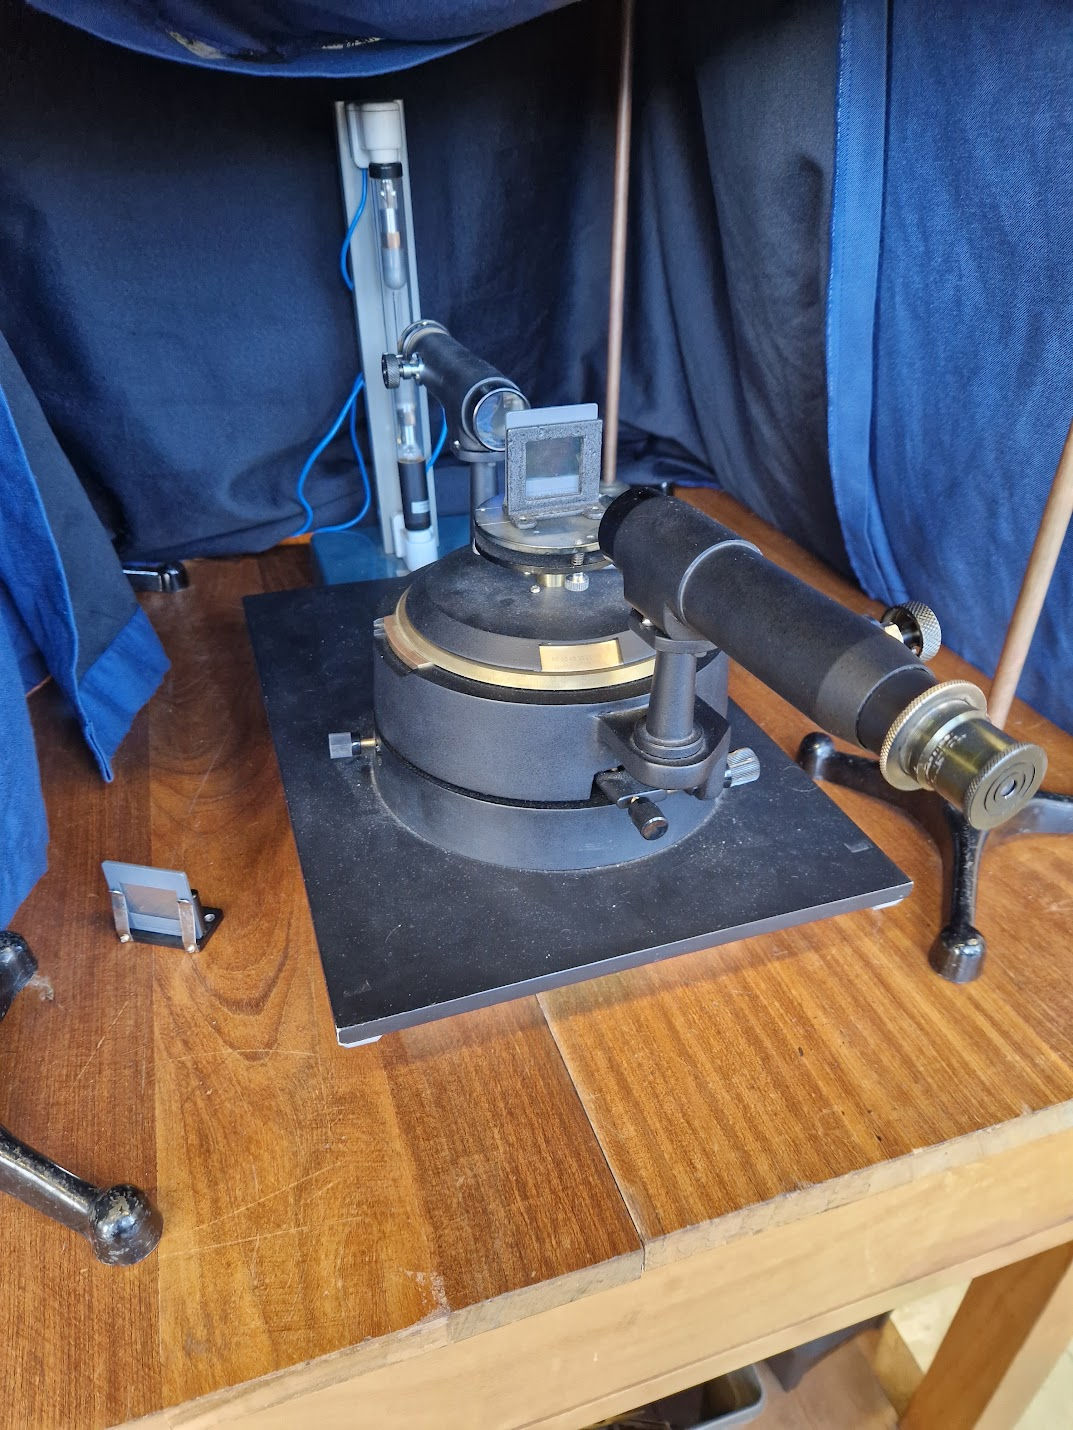
\includegraphics[width=0.5\textwidth]{images/Apparatus.png}
    \caption{Apparatus used for observing the Balmer spectrum of hydrogen.}
    \label{fig:apparatus}
\end{figure}

\begin{figure}[H]
    \centering
    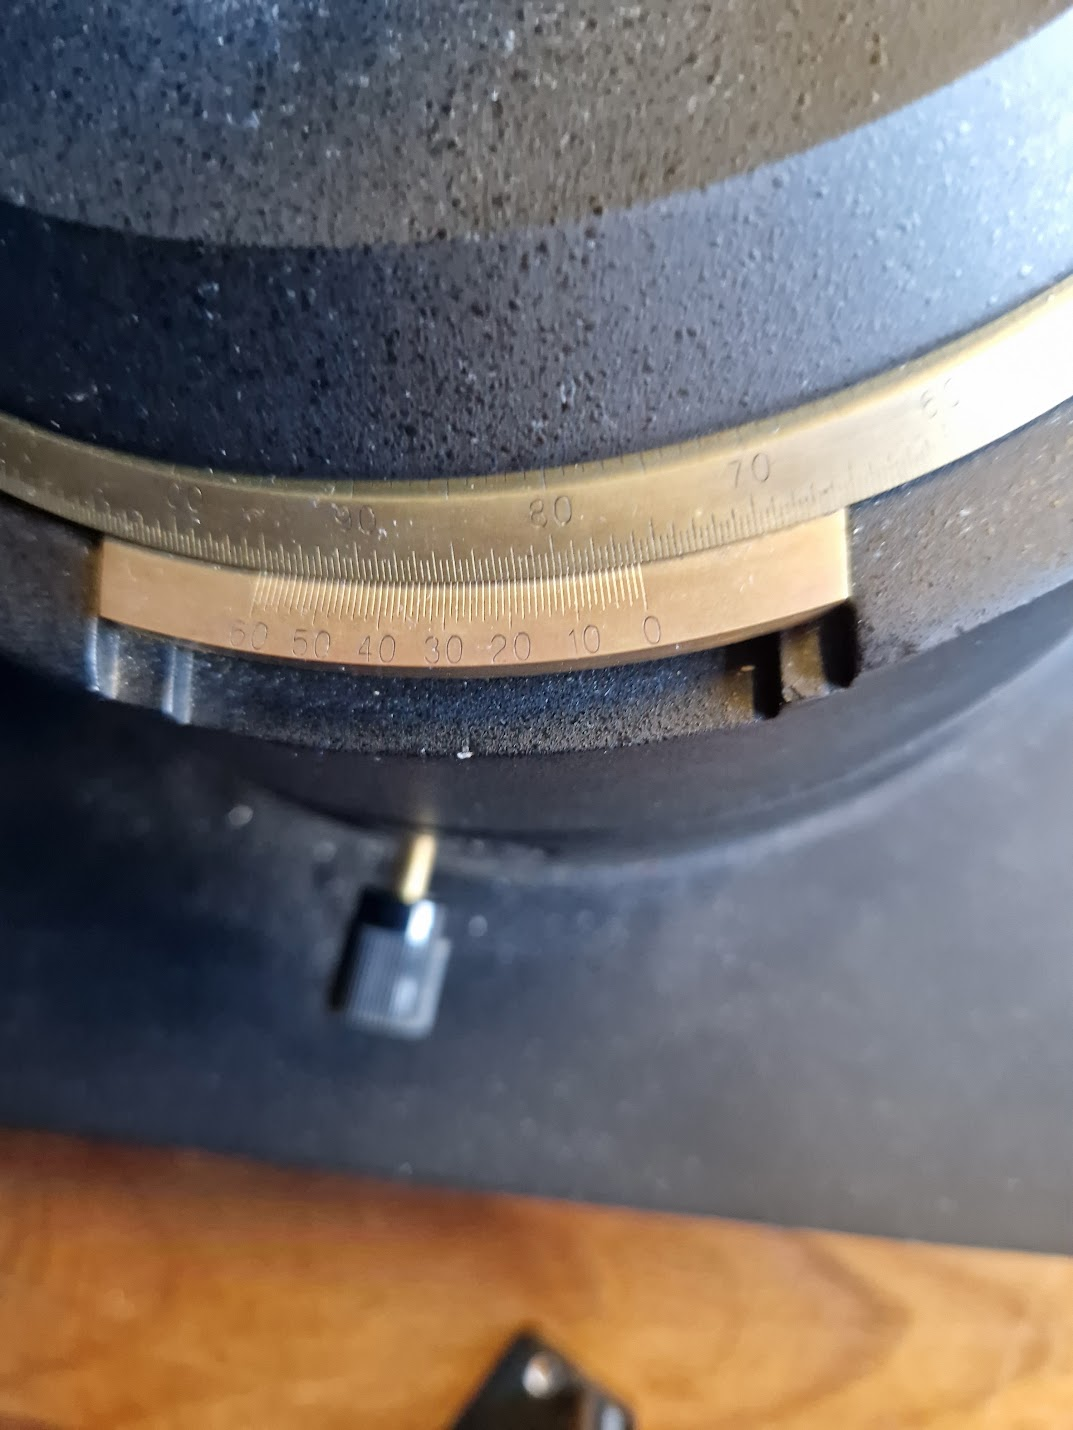
\includegraphics[width=0.5\textwidth]{images/Vernier.png}
    \caption{Vernier scale used for measuring diffraction angles.}
    \label{fig:vernier-scale}
\end{figure}

\begin{figure}[H]
    \centering
    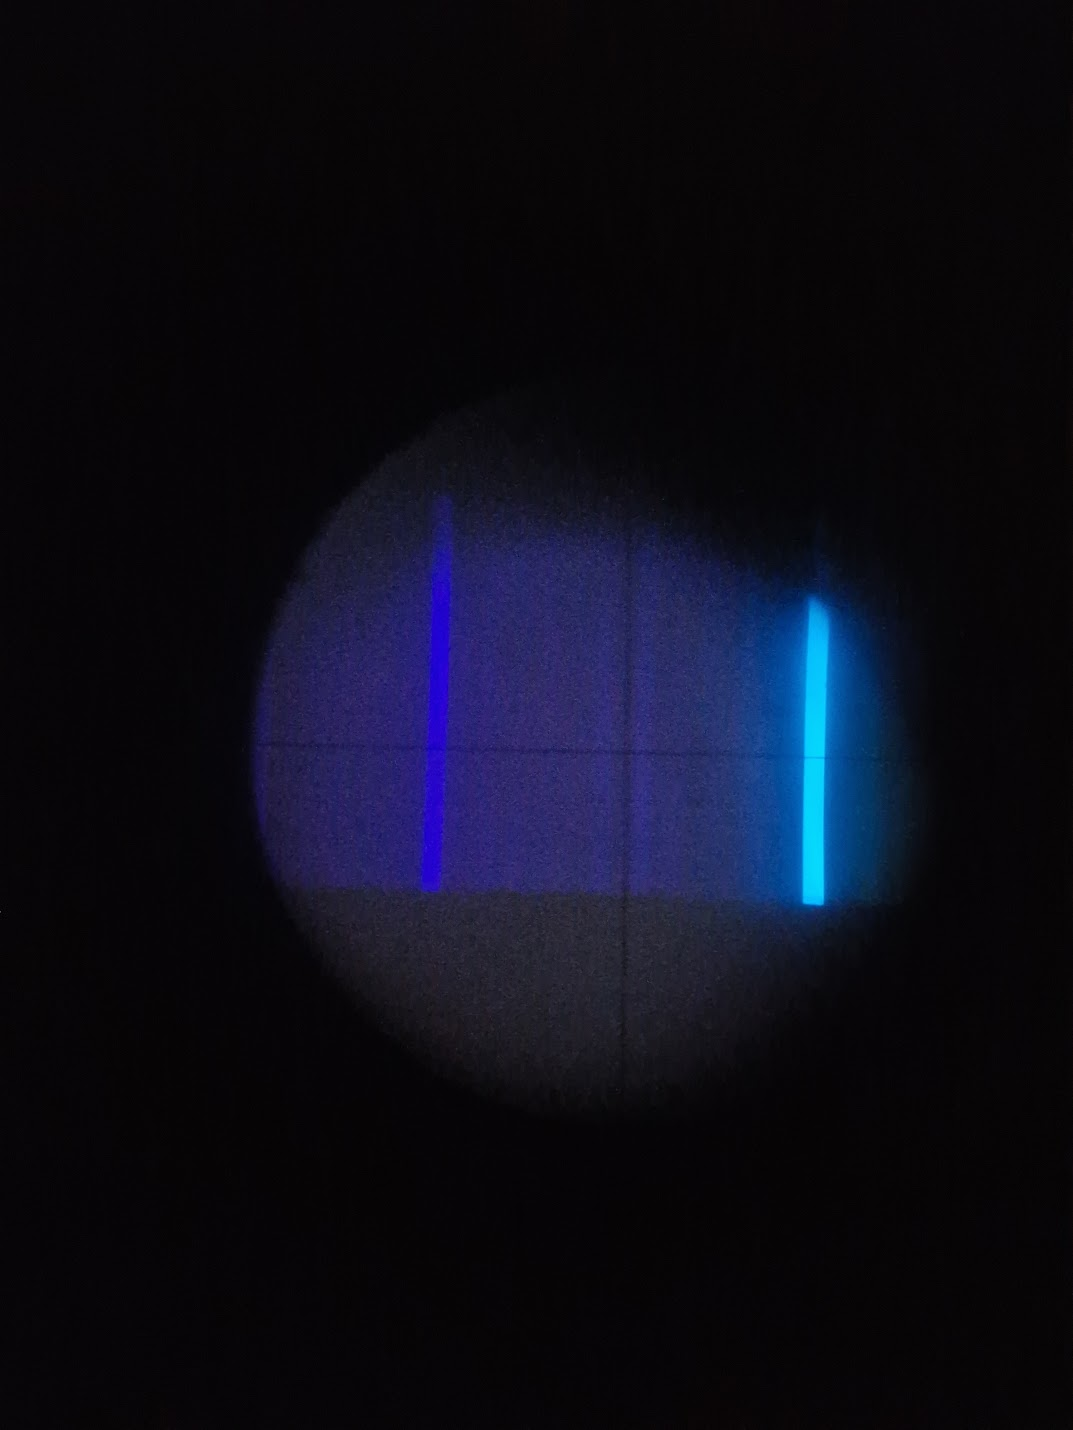
\includegraphics[width=0.5\textwidth]{images/Bands.png}
    \caption{Observed Balmer spectrum of hydrogen.}
    \label{fig:observed-bands}
\end{figure}

\newpage

%================================================
\section{Analysis}
%================================================

The grating had $600$ lines per millimetre, corresponding to
$d=1.667\times10^{-6}\ \si{\metre}$. The 14 usable measurements
comprise five observations of the $n_i=3$ line, four of $n_i=4$,
and five of $n_i=5$. Wavelengths were recalculated from the
recorded diffraction angles and orders. Table~\ref{tab:line-wavelengths}
summarises each line's mean, standard deviation, standard error
of the mean (SEM), and total uncertainty. The total uncertainty
combines the SEM and the assumed 1\% grating-spacing uncertainty
in quadrature.

\begin{table}[H]
    \centering
    \caption{Measured Balmer-line wavelengths and comparison
    with wavelengths calculated using the CODATA infinite-mass
    Rydberg constant \cite{nistRydberg}. The total uncertainty
    combines the SEM and the 1\% grating-spacing uncertainty;
    $\Delta/u$ is the difference from theory divided by this
    total uncertainty.}
    \label{tab:line-wavelengths}
    \small
    \begin{tabular}{cccccccc}
        \toprule
        Balmer line & Count & Mean (nm) & Std dev. (nm) &
        SEM (nm) & $\sigma_{\rm tot}$ (nm) & Theory (nm) & $\Delta/u$ \\
        \midrule
        H-$\alpha$ ($3\to2$) & 5 & 670 & 37 & 16.43 & 18 & 656.11 & 0.77 \\
        H-$\beta$ ($4\to2$) & 4 & 508 & 11 & 5.28 & 8 & 486.01 & 3.06 \\
        H-$\gamma$ ($5\to2$) & 5 & 448 & 12 & 5.16 & 7 & 433.94 & 1.99 \\
        \bottomrule
    \end{tabular}
\end{table}

As a check on the line identification, the Rydberg equation
predicts the H-$\alpha$ wavelength ($n_i=3\to n_f=2$) to be
\[
\lambda_{\alpha,\mathrm{theory}}
= \left[
R_\infty\left(\frac{1}{2^2}-\frac{1}{3^2}\right)
\right]^{-1}
= \left[
(1.0973731568\times10^7\ \si{\per\metre})
\left(\frac{5}{36}\right)
\right]^{-1}
= 656.11\ \si{\nano\metre}.
\]
The measured H-$\alpha$ mean is
$668\pm18\ \si{\nano\metre}$, a difference of
\SI{14}{\nano\metre} or 0.77 total uncertainties. The
measurement therefore agrees with the predicted value within
its stated uncertainty.

The fit variable was defined as
$x=1/n_f^2-1/n_i^2$, and the measured inverse wavelengths
were fitted to $y=mx+c$, where $y=1/\lambda$. The
unweighted least-squares fit gave

\[
m=(1.0292\pm0.0571)\times10^7\ \si{\per\metre},
\qquad
c=(6.129\pm10.0)\times10^4\ \si{\per\metre}.
\]

The slope is the experimental Rydberg constant. It is 6.21\%
below the infinite-mass reference value
$1.097373\times10^7\ \si{\per\metre}$ \cite{nistRydberg}.
The fitted intercept is consistent with zero within its
standard error. The fit and its extrapolation to the series
limit are shown in Figure~\ref{fig:balmer-fit}.

\begin{figure}[H]
    \centering
    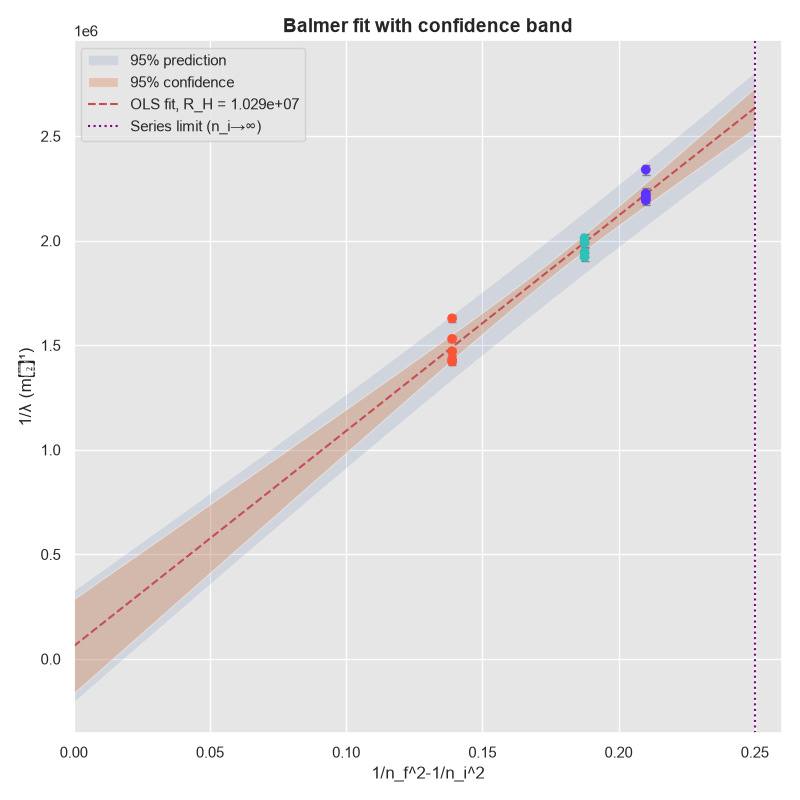
\includegraphics[width=0.86\textwidth]{images/balmer_fit_band.png}
    \caption{Inverse wavelength against
    $1/n_f^2-1/n_i^2$, with the unweighted linear fit and
    95\% confidence and prediction bands. The series limit
    occurs at $x=1/n_f^2=0.25$.}
    \label{fig:balmer-fit}
\end{figure}

For $n_i\rightarrow\infty$, $1/\lambda_{\mathrm{limit}}=R_H/4$.
Using the fitted slope gives

\[
\lambda_{\mathrm{limit}}=389\pm22\ \si{\nano\metre},
\qquad
E_{\mathrm{limit}}=3.2\pm0.2\ \si{\electronvolt}.
\]

The theoretical values calculated from the accepted Rydberg
constant are approximately \SI{364.5}{\nano\metre} and
\SI{3.401}{\electronvolt}, respectively \cite{nistRydberg}.
These uncertainties are propagated from the unweighted fit and
do not include the full systematic uncertainty.
The line-by-line reference wavelengths in
Table~\ref{tab:line-wavelengths} use $R_\infty$, matching the
analysis convention; the finite-proton-mass correction to the
hydrogen Rydberg constant is about 0.054\%.

The other plots provide checks on the line identification,
individual wavelength measurements, and regression
behaviour. The measured and theoretical wavelengths are
compared in Figure~\ref{fig:measured-theory}; the measured
spectrum and order-by-order wavelengths are shown in
Figures~\ref{fig:spectrum} and~\ref{fig:order-wavelength}.
Figure~\ref{fig:fit-comparison} compares the unweighted,
weighted, through-origin, and theoretical fits.

\begin{figure}[H]
    \centering
    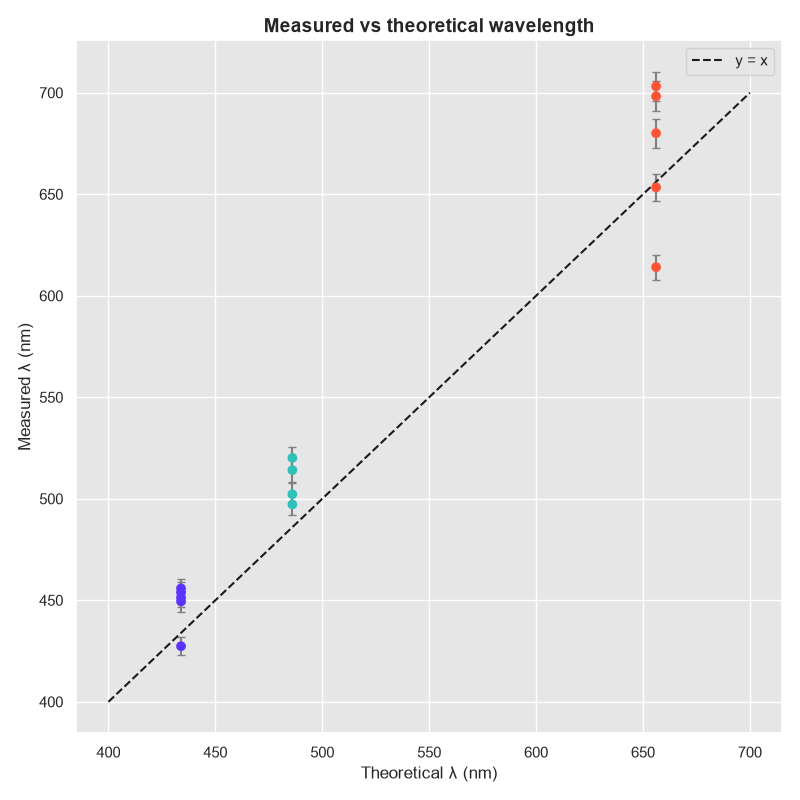
\includegraphics[width=0.72\textwidth]{images/measured_vs_theory.png}
    \caption{Measured wavelengths plotted against theoretical
    Balmer wavelengths. Error bars include the propagated
    angle uncertainty and the assumed grating-spacing
    uncertainty.}
    \label{fig:measured-theory}
\end{figure}

\begin{figure}[H]
    \centering
    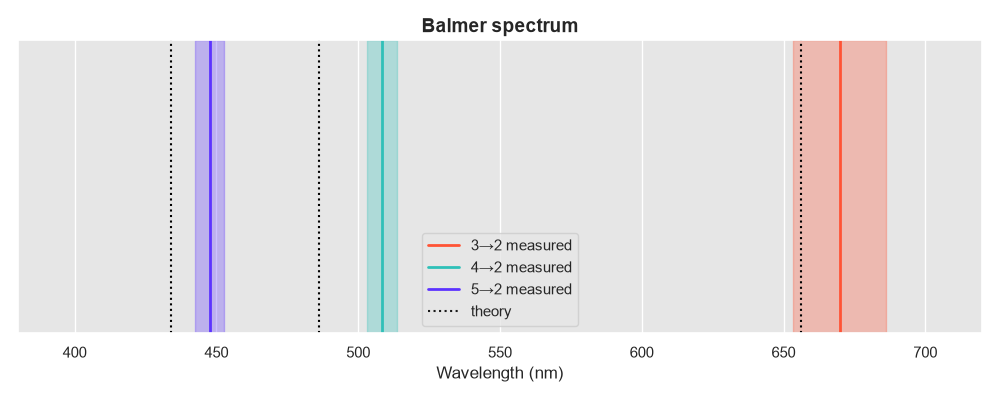
\includegraphics[width=0.82\textwidth]{images/spectrum.png}
    \caption{Measured Balmer-line positions compared with
    their theoretical wavelengths. H-$\alpha$, H-$\beta$,
    and H-$\gamma$ correspond to $n_i=3$, 4, and 5,
    respectively.}
    \label{fig:spectrum}
\end{figure}

\begin{figure}[H]
    \centering
    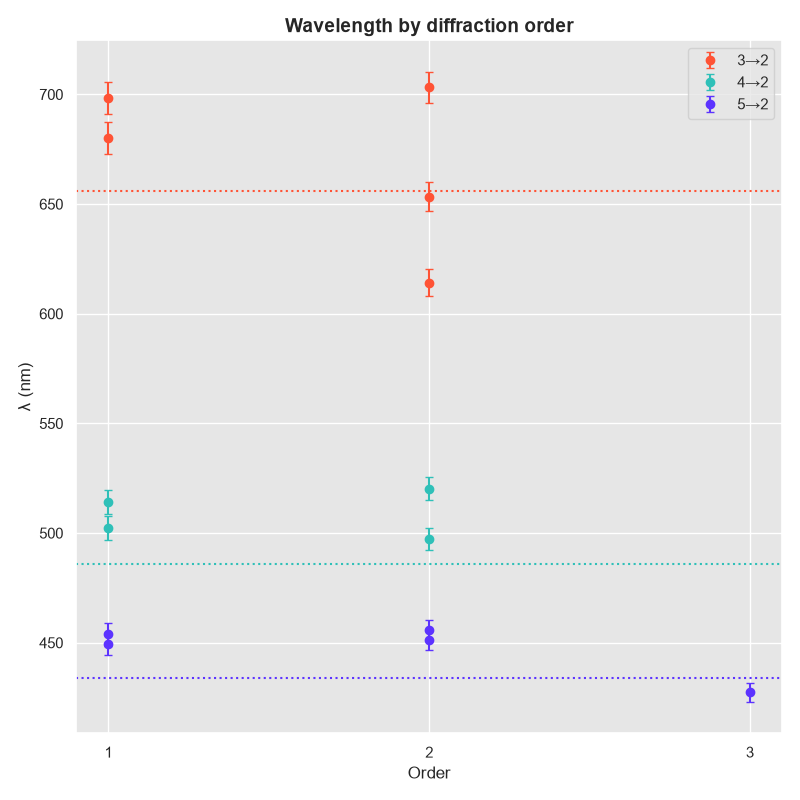
\includegraphics[width=0.82\textwidth]{images/lambda_by_order.png}
    \caption{Wavelength estimates for each Balmer line
    (H-$\alpha$, H-$\beta$, and H-$\gamma$) and diffraction
    order. Dotted lines indicate the theoretical wavelengths.}
    \label{fig:order-wavelength}
\end{figure}

\begin{table}[H]
    \centering
    \caption{Rydberg-constant estimates from alternative
    regressions. The weighted-fit uncertainty is formal; its
    goodness of fit indicates it is not an adequate
    description of the observed scatter.}
    \label{tab:fit-comparison}
    \begin{tabular}{lcc}
        \toprule
        Fit & $R_H$ ($10^7\ \si{\per\metre}$) &
        Reduced $\chi^2$ \\
        \midrule
        Unweighted, free intercept & $1.0292\pm0.0571$ & -- \\
        Weighted, free intercept & $1.0295\pm0.0160$ & 13.46 \\
        Weighted, forced through origin & $1.0631\pm0.0030$ & -- \\
        Infinite-mass reference \cite{nistRydberg} & 1.09737 & -- \\
        \bottomrule
    \end{tabular}
\end{table}

For the free-intercept weighted fit, $\chi^2=161.57$ for
12 degrees of freedom ($p<0.001$). The through-origin fit
differs from the reference value by 3.13\%, but its small
formal uncertainty does not reflect the excess scatter. A
bootstrap resampling of the 14 observations gives
$R_H=(1.030\pm0.064)\times10^7\ \si{\per\metre}$, with a
95\% interval from $8.976\times10^6$ to
$1.151\times10^7\ \si{\per\metre}$. The independent
intercept analysis gives $R_H/n_f^2=2.6343\times10^6\
\si{\per\metre}$ and an implied final level
$n_f=1.98\pm0.06$, consistent with the Balmer value of 2.
The bootstrap estimate for the final level is
$n_f=1.98\pm0.05$.
With the infinite-mass reference fixed and $n_f=2$, the
individually inferred initial levels have means (standard
deviations) of $2.97\ (0.11)$, $3.76\ (0.10)$, and
$4.67\ (0.31)$ for the three observed lines.

The fitted slope also corresponds to a Rydberg energy
$hcR_H=12.76\pm0.71\ \si{\electronvolt}$, compared with
\SI{13.61}{\electronvolt} from the reference value. The
estimated hydrogen-deuterium isotope shift at H-alpha is
\SI{0.18}{\nano\metre}. For an ideal grating illuminated over
\SI{2}{\centi\metre}, the resolving power
$\mathcal{R}=\eta N$ is 12\,000, 24\,000, and 36\,000 in
orders one to three, respectively; at \SI{656}{\nano\metre},
these correspond to nominal wavelength intervals of
\SI{0.055}{\nano\metre}, \SI{0.027}{\nano\metre}, and
\SI{0.018}{\nano\metre} \cite{openstaxDiffraction}. These are
ideal estimates, not measured resolution values.

\begin{figure}[H]
    \centering
    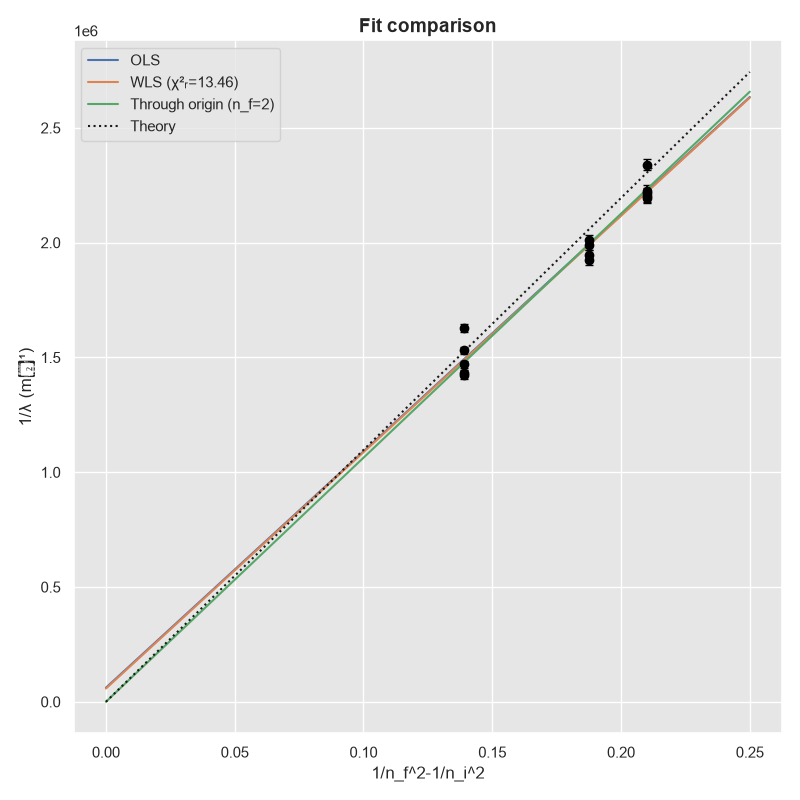
\includegraphics[width=0.82\textwidth]{images/fit_comparison.png}
    \caption{Comparison of regression models with the
    reference Rydberg slope. The free-intercept weighted
    fit has a reduced $\chi^2$ of 13.46.}
    \label{fig:fit-comparison}
\end{figure}

\newpage

%================================================
\section{Error Analysis}
%================================================

The wavelength uncertainty was estimated by propagating an
assumed angular reading uncertainty of
$\sigma_\theta=5$ arcminutes and a 1\% relative uncertainty in
the grating spacing. For
$\lambda=d\sin\theta/\eta$, the independent contributions
were combined as

\[
\sigma_\lambda =
\sqrt{
\left(\frac{d\cos\theta}{\eta}\sigma_\theta\right)^2
+\left(0.01\lambda\right)^2
},
\qquad
\sigma_{1/\lambda}=\frac{\sigma_\lambda}{\lambda^2}.
\]

The unweighted fit uncertainty is
$5.71\times10^5\ \si{\per\metre}$. The uncertainty budget
assigns $2.93\times10^4\ \si{\per\metre}$ to the angle
reading and approximately $1.03\times10^5\ \si{\per\metre}$
to the grating spacing. Thus, scatter in the
observations dominates the stated fit uncertainty, although
the grating calibration is a common systematic contribution
that does not average away over repeated measurements.

The weighted regression gives
$\chi^2=161.57$ for 12 degrees of freedom, corresponding
to a reduced $\chi^2=13.46$ and $p<0.001$ under the assumed
uncertainty model. The weighted-fit error
bars therefore substantially underestimate the dispersion
of the measurements, or the data contain additional
unmodelled effects. Consequently, the small formal weighted
uncertainty should not be interpreted as the accuracy of the
measurement. The residual diagnostics in
Figure~\ref{fig:residuals} show the deviations from the
unweighted fit.

\begin{figure}[H]
    \centering
    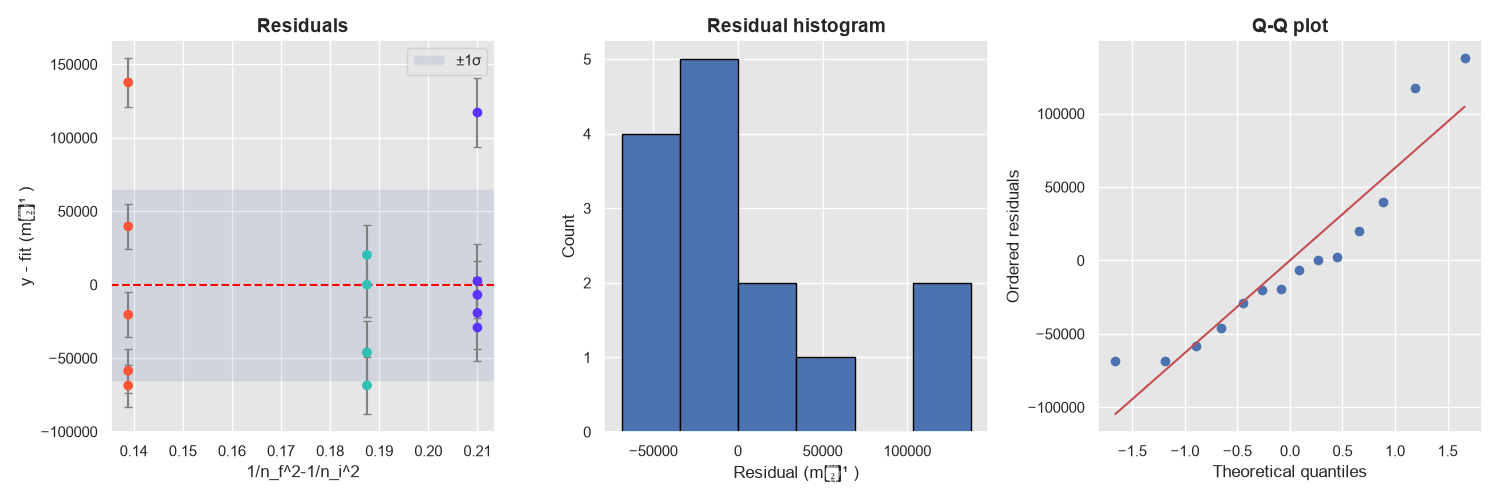
\includegraphics[width=\textwidth]{images/residual_diagnostics.png}
    \caption{Unweighted-fit residuals, their distribution,
    and a normal-probability plot. The residual scale is
    larger than expected from the propagated measurement
    uncertainties.}
    \label{fig:residuals}
\end{figure}

For the Rydberg constant, the unweighted fit gives
$R_H=(1.03\pm0.06)\times10^7\ \si{\per\metre}$, consistent
with the expected value within the experimental uncertainty.

The error was calculate as a combination of the propagated measurement uncertainties and the scatter in the observed wavelengths.

\[
    \sigma_\text{prop} = 5.71\times10^5\ \si{\per\metre},\quad
    \sigma_\text{scatter} = 1.03\times10^5\ \si{\per\metre},
\]

\[
\sigma_{R_H} = \sqrt{\sigma_\text{prop}^2 + \sigma_\text{scatter}^2} = 5.78\times10^5\ \si{\per\metre}
\]

\newpage

%================================================
\section{Discussion}

The observed wavelengths increase with decreasing
$n_i$, as expected for the Balmer series, and the fitted
gradient is about 1.2 unweighted-fit standard errors below
the infinite-mass reference value. The finite-mass hydrogen
value is about 0.054\% lower than this reference, a correction
that is small compared with the experimental uncertainty.
The fitted intercept is also consistent with zero. Together,
these results support the predicted linear relationship
between inverse wavelength and
$1/n_f^2-1/n_i^2$.

Each measured mean wavelength is longer than its theoretical
counterpart. The $n_i=3$ result agrees within one combined
standard uncertainty, while the $n_i=4$ result differs by
about 3.1 standard uncertainties and the $n_i=5$ result by
about 2.0. The consistent direction of the offsets suggests
that a common calibration or alignment effect may be present,
in addition to random uncertainty. Possible contributions
include uncertainty in locating the centre of a spectral
line, residual error in the straight-through reference,
grating alignment, and the assumed tolerance of the grating
spacing.

The weighted regression's large reduced chi-squared is
particularly important: the data are not described by the
stated independent-error model. This explains why forcing
the fit through the theoretically expected zero intercept
produces an apparently very precise result despite the
scatter. The unweighted fit, which reflects the observed
dispersion more directly, is therefore used for the reported
experimental value. The fit comparison and residual plots
make this limitation visible.

The series limit is an extrapolation from the three observed
lines to $n_i\rightarrow\infty$. Its uncertainty is
therefore relatively large, and the reported propagated
uncertainty does not fully represent the systematic and
model uncertainty. The $n_i=6$ transition was not included,
so an additional violet line could not provide another
independent point to constrain the fit. Future measurements
could improve the result by repeating both-side angle
readings, checking the angular zero and grating calibration,
and including additional visible orders and spectral lines.

\newpage

%================================================
\section{Conclusion}
%================================================

The Balmer spectrum was measured for transitions
$n_i=3,4,$ and $5$ to $n_f=2$. The unweighted fit gave
$R_H=(1.02\pm0.05)\times10^7\ \si{\per\metre}$, 6.21\%
below the infinite-mass reference value. The series-limit
wavelength was $389\pm22\ \si{\nano\metre}$. Although
the fitted intercept is consistent with zero and the
intercept analysis recovers a final level close to 2, the
weighted goodness-of-fit test ($\chi^2_\nu=13.46$) shows
that the stated measurement uncertainties do not account
for all the scatter. The measurements support the expected
Balmer-series relationship, but the precision is limited
by random scatter and systematic effects.

\newpage

%================================================
\section{References}
%================================================
\printbibliography
%================================================

\newpage

%================================================
\appendix

\section{Appendix}
\subsection{Data}
\begin{table}[!ht]
    \centering
    \caption{Recorded diffraction measurements and calculated
    wavelengths. The wavelength column is in metres.}
    \label{tab:raw-data}
    \begin{tabular}{ccccc}
        \toprule
        $band$ & $\eta$ & $\theta$ (rad) & $\sin\theta$ &
        $\lambda$ (m) \\
        \midrule
        \color{violet}$H-\gamma$ & 1 & 0.273027673 & 0.270 & $4.49\times10^{-7}$ \\
        \color{violet}$H-\gamma$ & 2 & 0.578848143 & 0.547 & $4.56\times10^{-7}$ \\
        \color{violet}$H-\gamma$ & 1 & 0.275781414 & 0.272 & $4.54\times10^{-7}$ \\
        \color{violet}$H-\gamma$ & 2 & 0.572293462 & 0.542 & $4.51\times10^{-7}$ \\
        \color{violet}$H-\gamma$ & 3 & 0.877726081 & 0.769 & $4.27\times10^{-7}$ \\
        \color{teal}$H-\beta$ & 1 & 0.306091966 & 0.301 & $5.02\times10^{-7}$ \\
        \color{teal}$H-\beta$ & 2 & 0.674065550 & 0.624 & $5.20\times10^{-7}$ \\
        \color{teal}$H-\beta$ & 1 & 0.313596881 & 0.308 & $5.14\times10^{-7}$ \\
        \color{teal}$H-\beta$ & 2 & 0.639294712 & 0.597 & $4.97\times10^{-7}$ \\
        \color{red}$H-\alpha$ & 1 & 0.420314069 & 0.408 & $6.80\times10^{-7}$ \\
        \color{red}$H-\alpha$ & 2 & 0.901191063 & 0.784 & $6.53\times10^{-7}$ \\
        \color{red}$H-\alpha$ & 1 & 0.432279271 & 0.419 & $6.98\times10^{-7}$ \\
        \color{red}$H-\alpha$ & 2 & 0.828469011 & 0.737 & $6.14\times10^{-7}$ \\
        \color{red}$H-\alpha$ & 2 & 1.004320629 & 0.844 & $7.03\times10^{-7}$ \\
        \bottomrule
    \end{tabular}
\end{table}

\subsection{Hydrogen energy levels from the Schr\"odinger equation}

The separation of the hydrogen Schr\"odinger equation into
radial and angular parts follows the standard treatment of the
hydrogen atom \cite{openstaxHydrogen}. In the non-relativistic
model, the electron and proton interact through the Coulomb
potential:

\[
    V(r) = \frac{-e^2}{4 \pi \epsilon_0 r}
\]

Here, $e$ is the elementary charge and $\epsilon_0$ is the
permittivity of free space. Using the reduced mass $m_r$ for
the electron--proton system, the time-independent Schr\"odinger
equation is

\[
    -\frac{\hbar^2}{2m_r} \nabla^2 \psi(r) + V(r) \psi(r) = E \psi(r)
\]

Because the potential depends only on the distance $r$ from the
nucleus, the wavefunction can be separated into a radial part
and an angular part:

\[
    \psi(r, \theta, \phi) = R(r) Y(\theta, \phi)
\]

The angular dependence is described by the angular-momentum
operator. Its eigenfunctions are spherical harmonics, with
eigenvalues $l(l+1)\hbar^2$:

\[
    \hat{L}^2 = -\hbar^2 \left[ \frac{1}{\sin\theta} \frac{\partial}{\partial \theta} \left( \sin\theta \frac{\partial}{\partial \theta} \right) + \frac{1}{\sin^2\theta} \frac{\partial^2}{\partial \phi^2} \right]  
\]

In spherical coordinates, the Laplacian can be written in
terms of the radial derivative and this angular-momentum
operator:

\[
    \nabla^2 = \frac{1}{r^2} \frac{\partial}{\partial r} \left( r^2 \frac{\partial}{\partial r} \right) - \frac{\hat{L}^2}{\hbar^2 r^2}
\]

\[
    -\frac{\hbar^2}{2m_r} \left[ \frac{1}{r^2} \frac{d}{dr} \left( r^2 \frac{dR(r)}{dr} \right) - \frac{l(l+1)}{r^2} R(r) \right] + V(r) R(r) = E R(r)
\]

Dividing out the angular function leaves an equation involving
only $r$. The term proportional to $l(l+1)$ is the centrifugal
contribution to the effective radial potential. A standard
substitution removes the first-derivative term:

\[
    u(r) = r R(r)
\]

With this substitution, the radial equation takes the
one-dimensional form

\[
    -\frac{\hbar^2}{2m_r} \frac{d^2 u(r)}{dr^2} + \left[ V(r) + \frac{l(l+1)\hbar^2}{2m_r r^2} \right] u(r) = E u(r)
\]

For bound states the energy is negative, $E<0$, and the radial
wavefunction must remain finite at the origin and decay at large
$r$. It is useful to define a positive decay constant $k$ and
a dimensionless radial coordinate $\rho$:

\[
    k = \frac{\sqrt{-2m_r E}}{\hbar}
\]

and

\[
    \rho = 2 k r
\]

The acceptable solution behaves as shown at the two boundaries:

\[
    r = 0,\quad u \approx r^{l+1}
\]

\[
    r \to \infty, \quad u \approx e^{-k r}
\]

Factoring out both limiting behaviours leaves a function $L$
that is represented by a power series:

\[
    u(\rho) = \rho^{l+1} e^{-\rho/2} L(\rho)
\]

Unless this series terminates, it grows at large $r$ and the
wavefunction is not normalisable. Requiring termination
quantises the energy; the resulting integer $n$ is the principal
quantum number, with $n\geq l+1$:

\[
    n = \frac{e^2}{4 \pi \epsilon_0 \hbar}
    \sqrt{\frac{m_r}{-2E}}
\]

\[
    k = \frac{m_r e^2}{4 \pi \epsilon_0 \hbar^2 n}
\]

Substituting this allowed value of $k$ into $E=-\hbar^2 k^2/(2m_r)$
gives the discrete energy levels:

\[
    E_n = -\frac{m_r e^4}{2 (4 \pi \epsilon_0)^2 \hbar^2 n^2}
\]

\[
    E_n = -\frac{13.6 \text{ eV}}{n^2}
\]

When an electron drops from an initial level $n_i$ to a lower
level $n_f$, the emitted photon carries the energy difference
$E_{n_i}-E_{n_f}$. Using the photon relations $E_\gamma=hf$
and $f=c/\lambda$, this energy difference gives the wavelength:

\[
    hf = E_{n_i}-E_{n_f},
    \qquad
    \lambda = \frac{c}{f}
\]

Substituting the quantised energy levels into this relation
gives the Rydberg formula:

\[
    \frac{1}{\lambda}
    = R_H \left( \frac{1}{n_f^2} - \frac{1}{n_i^2} \right),
    \qquad
    R_H = \frac{m_r e^4}{8\epsilon_0^2 h^3 c}
    = 1.096776\times10^7\ \si{\per\metre}
\]

For the Balmer series, $n_f=2$. The predicted wavelengths for
the three visible transitions measured in this experiment are
therefore:

\[
    \begin{aligned}
        \lambda_{\mathrm{H}\alpha}\ (3\to2)
        &= \left[R_H\left(\frac{1}{2^2}-\frac{1}{3^2}\right)\right]^{-1}
        = 6.565\times10^{-7}\ \si{\metre}
        = 656.5\ \si{\nano\metre},\\
        \lambda_{\mathrm{H}\beta}\ (4\to2)
        &= \left[R_H\left(\frac{1}{2^2}-\frac{1}{4^2}\right)\right]^{-1}
        = 4.863\times10^{-7}\ \si{\metre}
        = 486.3\ \si{\nano\metre},\\
        \lambda_{\mathrm{H}\gamma}\ (5\to2)
        &= \left[R_H\left(\frac{1}{2^2}-\frac{1}{5^2}\right)\right]^{-1}
        = 4.342\times10^{-7}\ \si{\metre}
        = 434.2\ \si{\nano\metre}.
    \end{aligned}
\]

\end{document}